\chapter{UML: Aktivitätsdiagramm}\label{ch:uml_act}
Das Aktivitätsdiagramm zeigt die Abläufe und Prozesse, die in unserem Projekt stattfinden.
In Abbildung ~\ref{fig:act} ist das Aktivitätsdiagramm für unser Projekt dargestellt und zeigt alle Aktivitäten in 
abstrahierter Form zur besseren Verständlichkeit. \\
\newline
Die dargestellte Aktivität dieses Diagramms ist das Gewinnen eines Topfskins durch den Nutzer.
Der Nutzer kann im Menü das Potpack auswählen und es bedingt kaufen.


\vspace{1cm}
\begin{figure}[h]
    \centering
    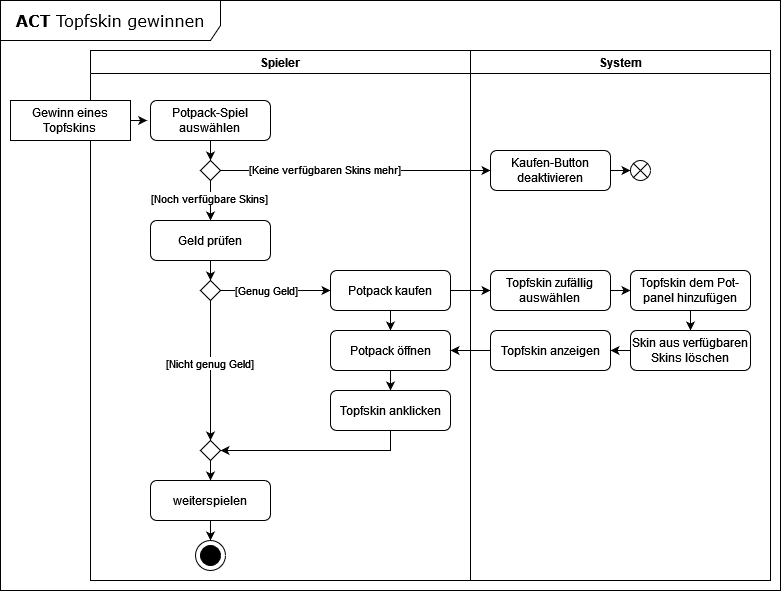
\includegraphics[width=\linewidth]{../bilder/act_potpack}
    \vspace{0.05cm}
    \caption{Aktivitätsdiagramm}
    \label{fig:act}
\end{figure}